\begin{frame}
    \begin{center}
    \begin{tabular}{ccc}
        \visible<1->{
\includegraphics[width=0.3\linewidth]{figures/platypus.pdf}} &
        \visible<2->{ \Huge VS} &
        \visible<3->{
\includegraphics[width=0.3\linewidth]{figures/wa-logo-stacked2-large.png}}
    \end{tabular}
    \end{center}
\end{frame}

\section{Concluons !}

\subsection{Projets}

\begin{frame}
    \frametitle{Plus de résultats}

    Pas de réponse via \alert{Wikidata}:
    \begin{itemize}
      \item ``Quel est la vitesse du TGV?''
      \item ``Quand est ouvert le supermarché le plus proche ?''
    \end{itemize}

    \pause
    \medbreak

    $\rightarrow$ Améliorer Wikidata?

    $\rightarrow$ Utiliser d'autres bases de données comme \alert{OpenStreeMap} ?
\end{frame}

\begin{frame}
    \frametitle{Autres projets...}

    \begin{itemize}
        \item Support d'autre langues (French...)
        \item Améliorer l'expérience utilisateur
    \end{itemize}
    
    \pause
     \medbreak

    $\rightarrow$ On a besoin de vous !
\end{frame}

\subsection{Conclusion}

\begin{frame}
    \frametitle{Platypus ?}

    \begin{itemize}
        \item Un \textit{framework} open-source de réponse aux questions
        \item Une démo déjà utilisable, \alert{Platypus}
    \end{itemize}
\end{frame}


\newlength{\logosize}
\setlength{\logosize}{12pt}
\begin{frame}
    \frametitle{Questions?}  
    \begin{columns}
    \begin{column}{0.55\textwidth}
        \alert{\url{http://projetpp.github.io}}\vspace{5pt}
        \begin{tabular}{ll}
            
\includegraphics[width=\logosize]{Twitter_logo_blue.png} & \href{https://twitter.com/ProjetPP}{https://twitter.com/ProjetPP}\\
            
\includegraphics[width=\logosize]{GitHub-Mark-32px.png} &  \href{https://github.com/ProjetPP}{https://github.com/ProjetPP}\\
            
\includegraphics[width=\logosize]{figures/forum.png} &  \href{http://discourse.askplatyp.us}{http://discourse.askplatyp.us}\\
            
\includegraphics[width=\logosize]{ic_email_black_18dp.png} & \href{mailto:askplatyp.us}{contact@askplatyp.us}\\
        \end{tabular}
    \end{column}
    \begin{column}{0.5\textwidth}
        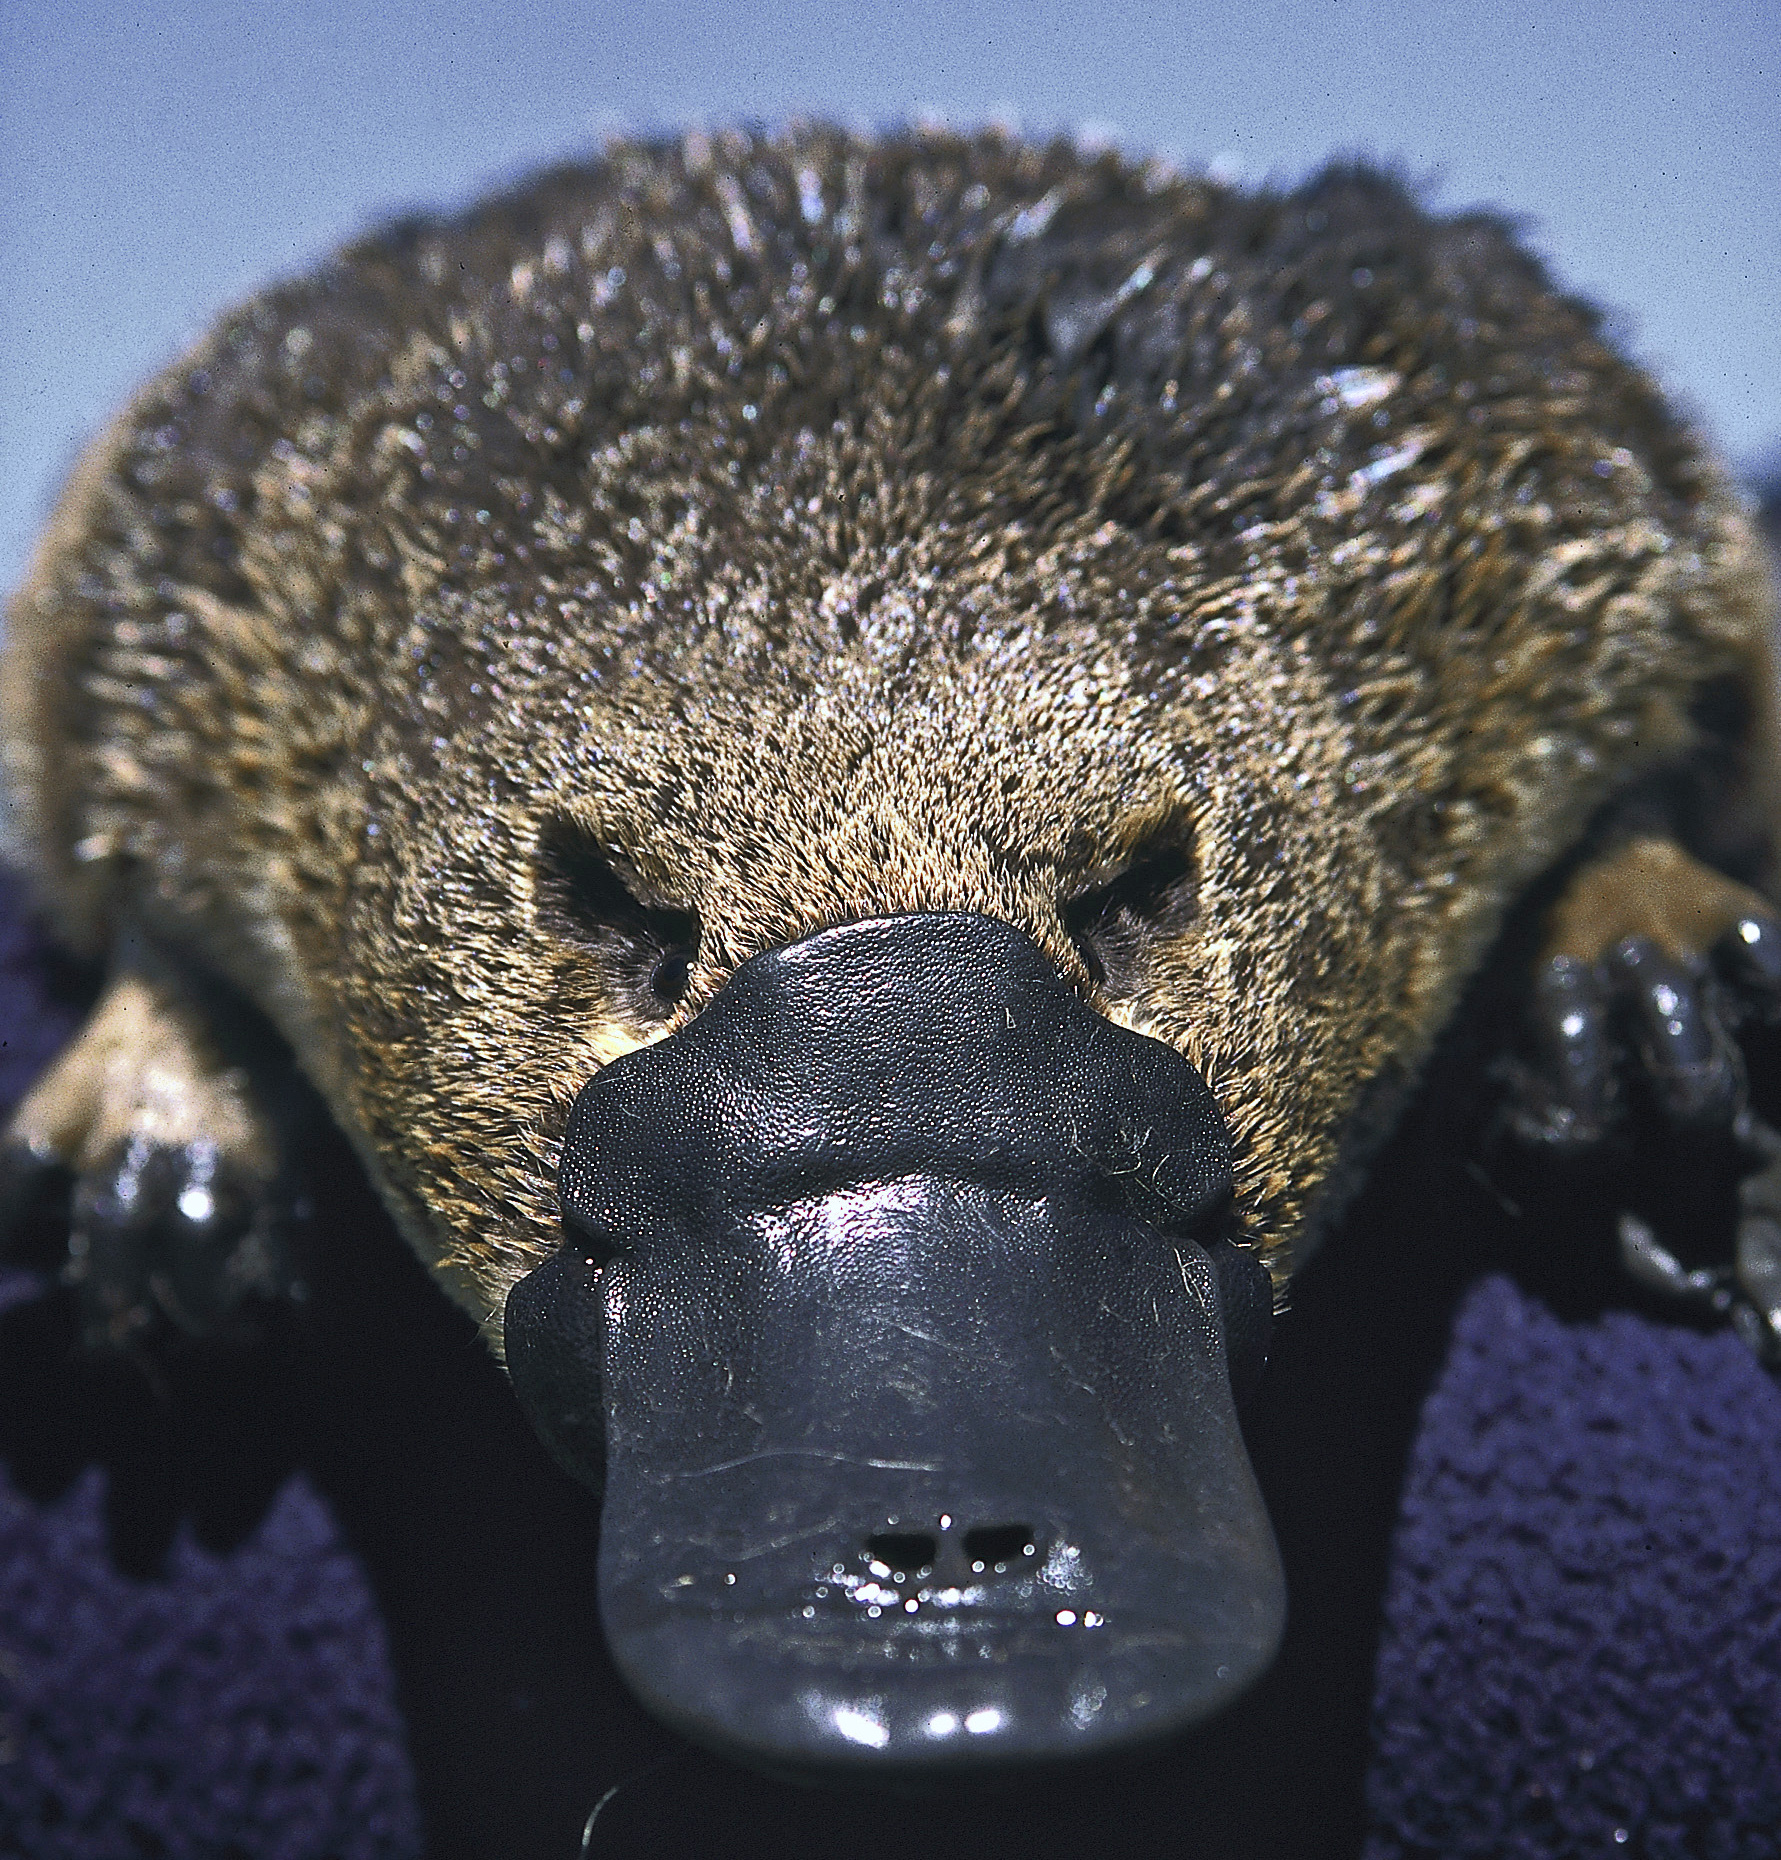
\includegraphics[width=\linewidth]{figures/Ornithorhynchus.jpg}
    \end{column}
    \end{columns}
\end{frame}

%\iffalse
\begin{frame}
    \begin{center}
        \Huge Demo time!
    \end{center}
\end{frame}

\begin{frame}[plain]
    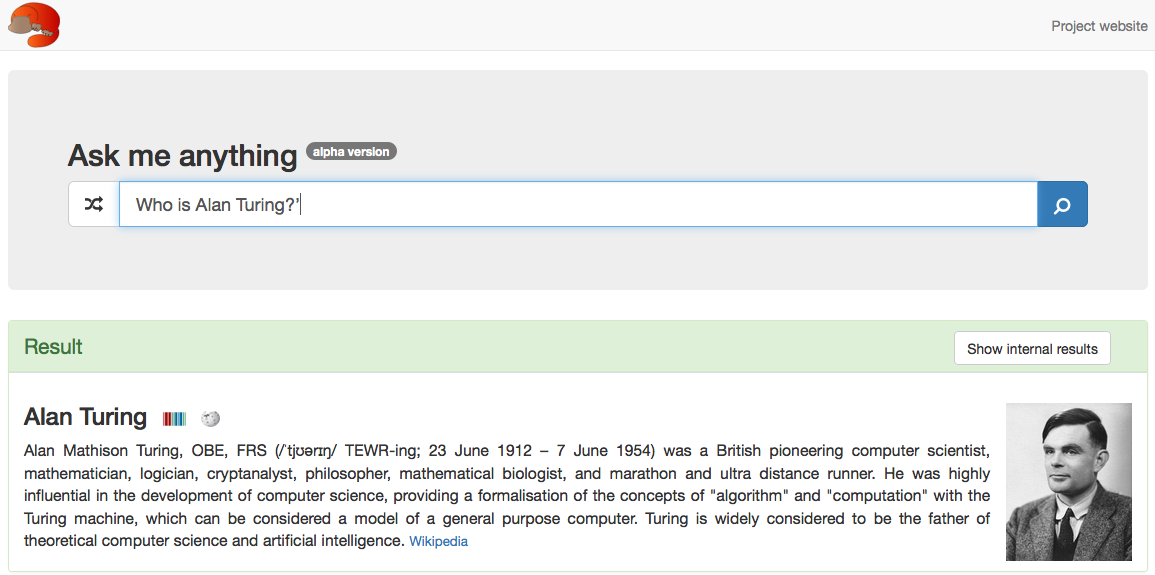
\includegraphics[width=\linewidth]{figures/demo-whoIsAlanTuring.png}
\end{frame}

\begin{frame}[plain]
    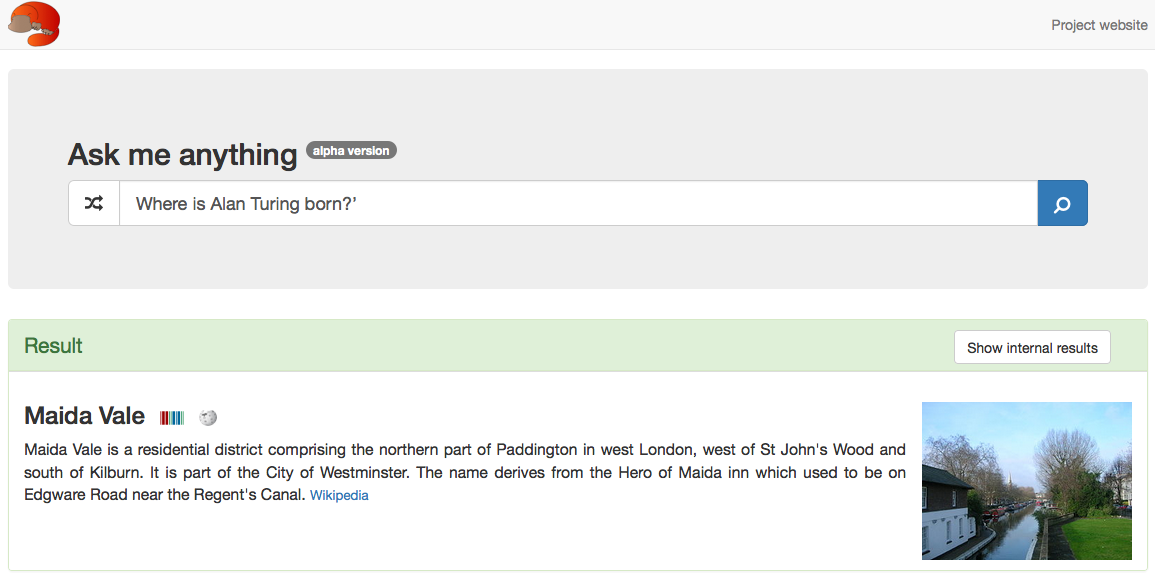
\includegraphics[width=\linewidth]{figures/demo-whenIsAlanTuringBorn.png}
\end{frame}

\begin{frame}[plain]
    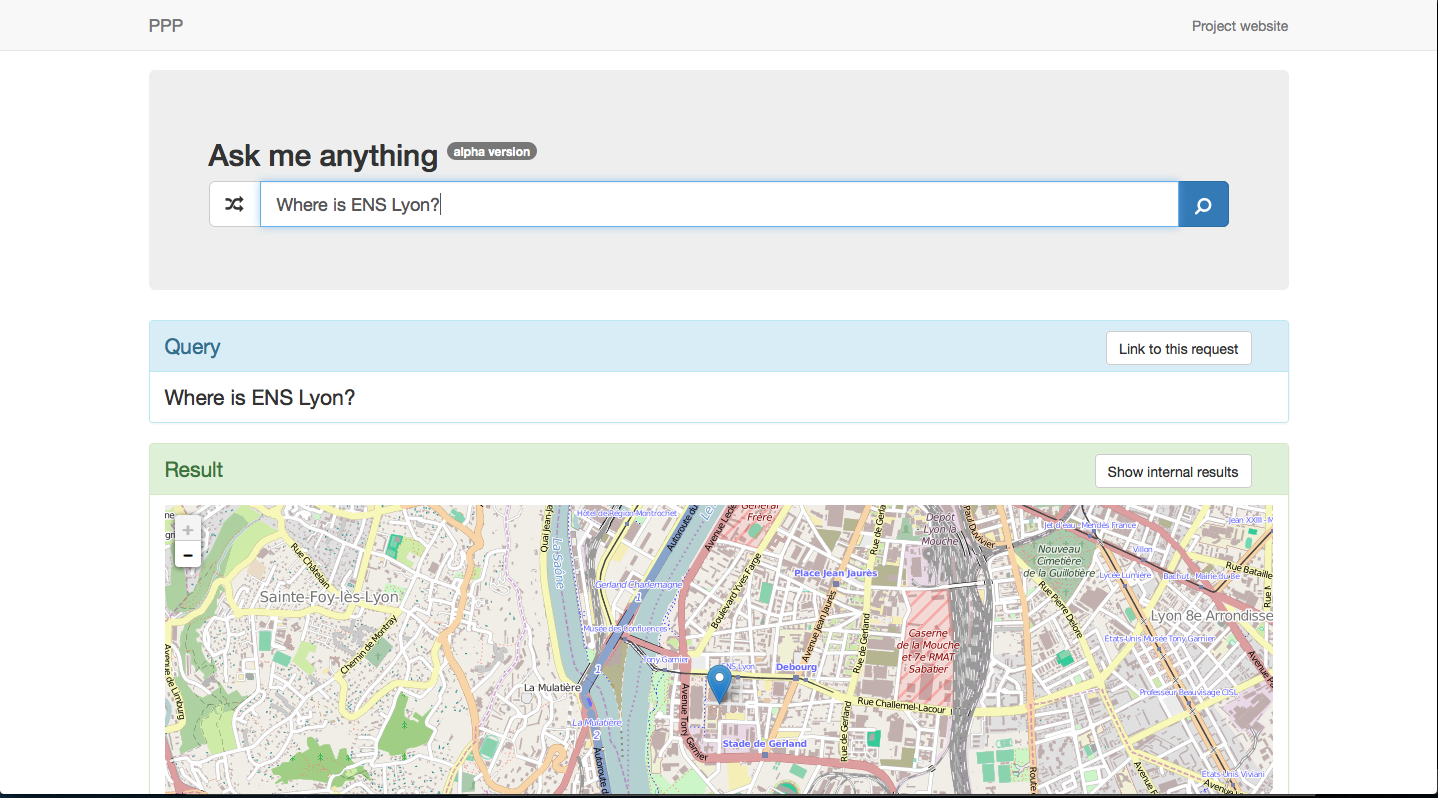
\includegraphics[width=\linewidth]{figures/demo-whereIsEnsLyon.png}
\end{frame}

\begin{frame}
    \begin{center}
    \begin{tabular}{ccc}
        
\includegraphics[width=0.3\linewidth]{figures/platypus.pdf} &
        \Huge VS &
        
\includegraphics[width=0.3\linewidth]{figures/wa-logo-stacked2-large.png}
    \end{tabular}
    \end{center}
\end{frame}


\begin{frame}
    \frametitle{Nested question}

Who is the wife of the president of the United States?
    \begin{tabular}{ll}
        \alert{WolframAlpha} & Barack Obama\\
        \alert{Platypus} & Michelle Obama\\
    \end{tabular}

    \medbreak

    \onslide<2->{
        What are the birth dates of the daughters of the wife of the president of the United States?
        \begin{tabular}{ll}
            \alert{WolframAlpha} & Barack Obama\\
            \alert{Platypus} & Saturday, July 4, 1998 \& Sunday, June 10, 2001\\
        \end{tabular}
    }
\end{frame}

\begin{frame}
    \frametitle{Conjunction}

Who is the actor of Inception and Titanic?
    \begin{tabular}{ll}
        \alert{WolframAlpha} & all the actors of the two movies\\
        \alert{Platypus} & Leonardo DiCaprio\\
    \end{tabular}
\end{frame}